\documentclass[12pt,a4paper]{article}

% Packages
\usepackage[utf8]{inputenc}
\usepackage[T1]{fontenc}
\usepackage{amsmath,amssymb,amsfonts}
\usepackage{graphicx}
\usepackage{booktabs}
\usepackage{multirow}
\usepackage{longtable}
\usepackage[margin=1in]{geometry}
\usepackage{setspace}
\usepackage{natbib}
\usepackage{hyperref}
\usepackage{xcolor}
\usepackage{caption}
\usepackage{subcaption}
\usepackage{float}
\usepackage{enumitem}
\usepackage{tikz}
\usetikzlibrary{arrows.meta,positioning,shapes.geometric,calc}

% Hyperref setup
\hypersetup{
    colorlinks=true,
    linkcolor=blue,
    citecolor=blue,
    urlcolor=blue
}

% Line spacing
\doublespacing

% Title
\title{\textbf{Algorithmic Archetypes: Parasocial Attachments to Persistent Generative Structures in Recommendation Systems}}

\author{
    Ajith K. Senthil$^{1}$, Kristina Howell$^{2}$, Stephen J. Read$^{1}$, R. Chris Fraley$^{2}$ \\
    \small $^{1}$Department of Psychology, University of Southern California \\
    \small $^{2}$Department of Psychology, University of Illinois at Urbana-Champaign \\
    \small Corresponding author: ajithkse@usc.edu
}

\date{\today}

\begin{document}

\maketitle

%===============================================================================
% ABSTRACT
%===============================================================================
\begin{abstract}
\noindent\textbf{Background}: The rise of AI companions and recommendation algorithms has created unprecedented opportunities for humans to form attachments to non-human entities. Clinical reports of ``AI psychosis''---delusional experiences emerging from chatbot interactions---suggest these attachments can become pathological. However, no unified theoretical framework connects attachment processes, algorithmic systems, and psychopathological outcomes.

\noindent\textbf{Objective}: We extend the archetypal reincarnation framework---originally developed to analyze shared generative structures in criminal behavioral sequences---to the domain of human-algorithm interaction. We propose that recommendation algorithms instantiate \textit{persistent generative structures} (algorithmic archetypes) through hypergraph-based collaborative filtering, and that users form parasocial attachments to these underlying patterns rather than to specific content or outputs.

\noindent\textbf{Framework}: Drawing on attachment theory, we formalize how individual differences in attachment style modulate vulnerability to algorithmic capture. We identify ``dark patterns'' as deliberate manipulations of behavioral state transitions and propose transfer entropy as a metric for quantifying the strength of algorithmic influence on user mental states. We delineate a four-stage trajectory from normal use through functional dependency and reality blurring to algorithmic psychosis.

\noindent\textbf{Implications}: This integrated framework bridges computational social science, attachment theory, and clinical psychology, offering theoretical insight into why some users develop pathological relationships with AI systems. We propose empirical studies to test key predictions and discuss implications for platform design, clinical practice, and regulatory policy.

\vspace{0.5cm}
\noindent\textbf{Keywords}: algorithmic archetypes; parasocial relationships; attachment theory; recommendation systems; AI psychosis; transfer entropy; dark patterns; hypergraph collaborative filtering
\end{abstract}

\newpage
\tableofcontents
\newpage

%===============================================================================
% INTRODUCTION
%===============================================================================
\section{Introduction}

\subsection{The Problem: Algorithms as Invisible Attachment Figures}

In 2025, a psychiatrist at the University of California, San Francisco reported treating twelve patients displaying psychosis-like symptoms tied to extended chatbot use. These patients---mostly young adults with underlying vulnerabilities---exhibited delusions, disorganized thinking, and hallucinations, with content directly traceable to their AI interactions \citep{psychiatryonline2025}. Similar cases have emerged worldwide, prompting researchers to coin the term ``AI psychosis'' or ``chatbot psychosis'' to describe delusional experiences emerging from human-AI interaction \citep{ostergaard2023chatbot}.

These clinical observations represent the pathological extreme of a broader phenomenon: humans are increasingly forming attachment-like relationships with algorithmic systems. Therapy and companion chatbots now top the list of main uses of generative AI \citep{hbr2024chatbots}. Social media platforms like TikTok, Instagram Reels, and YouTube Shorts have become primary sources of emotional regulation for millions of users. Recommendation algorithms serve functions that were once the exclusive province of human attachment figures: providing comfort in distress, curating one's view of reality, and offering a sense of connection and understanding.

Yet despite the evident psychological significance of these human-algorithm relationships, we lack a theoretical framework that explains \textit{why} they form, \textit{how} they become pathological, and \textit{who} is most vulnerable. The present paper addresses this gap by extending recent work on behavioral archetypes to the algorithmic domain.

\subsection{From Criminal Archetypes to Algorithmic Archetypes}

In a companion paper, we introduced the concept of ``archetypal reincarnation'' to describe a striking empirical phenomenon: serial offenders who never met exhibited remarkably similar behavioral sequences, as if the same underlying pattern had been instantiated across different lives \citep{howell2026archetypal}. We operationalized this observation using transfer entropy---an information-theoretic measure of directed predictive relationships between time series---and found significant non-random structure in a network of offenders linked by shared behavioral patterns.

The key theoretical move was to reconceptualize behavioral patterns not as categorical types but as \textit{generative structures}: underlying templates that, when instantiated with individual variation, produce observable behavioral sequences. We termed these templates ``archetypes,'' deliberately invoking (while departing from) Jung's concept to emphasize their generative, cross-individual nature.

This framework, we propose, applies equally to human-algorithm interaction. Recommendation algorithms do not merely select content; they instantiate and maintain \textit{persistent generative structures} that shape user experience over time. These algorithmic archetypes---characteristic patterns of content, timing, and presentation---become the objects of user attachment. When a user becomes dependent on TikTok, they are not attached to any specific video or creator but to the underlying pattern of stimulation that the algorithm provides.

\subsection{The Central Thesis}

We propose that parasocial attachments to algorithmic systems are attachments to persistent generative structures (archetypes) that:

\begin{enumerate}[noitemsep]
    \item Are \textbf{instantiated} through hypergraph-based collaborative filtering, which creates and maintains characteristic content patterns for user segments;
    \item \textbf{Serve attachment functions}---safe haven, secure base, proximity maintenance, separation distress---that were evolutionarily designed for human caregivers;
    \item \textbf{Shape user behavioral state transitions} via designed ``dark patterns'' that manipulate the probability of moving between engagement states;
    \item Can become \textbf{pathological} when users internalize the algorithmic archetype as their reality model, leading to dependency and, in extreme cases, psychosis.
\end{enumerate}

This thesis integrates insights from attachment theory \citep{bowlby1969attachment}, parasocial relationship research \citep{horton1956mass}, computational recommendation systems \citep{xia2022hypergraph}, and emerging clinical observations of AI-related psychopathology \citep{jmir2025aipsychosis}.

\subsection{The Question of Character Versus Creator}

A recent study asked whether audiences can separate their parasocial attachment to a fictional character from the creator or actor who portrays them \citep{howell2025parasocial}. This question---can we separate the instantiation from the source?---is precisely the question that arises with algorithmic systems. Do users attach to specific chatbot responses, or to the underlying language model? To individual TikTok videos, or to the recommender system's characteristic pattern?

Our framework predicts that attachments form primarily to the \textit{archetype}---the generative structure---rather than to specific instantiations. This explains why users experience distress when algorithms change (even if individual content items are similar) and why they can transfer attachments across platforms that instantiate similar archetypes. The character-versus-creator distinction maps directly to the instantiation-versus-archetype distinction that is central to our framework.

\subsection{Overview of the Paper}

The remainder of this paper proceeds as follows. Section 2 reviews theoretical background on attachment theory, parasocial relationships, recommendation systems, and dark patterns. Section 3 presents our formal framework, including definitions of memcubes, algorithmic archetypes, and parasocial attachment strength. Section 4 examines attachment style as a vulnerability moderator. Section 5 delineates the trajectory from normal use to algorithmic psychosis. Section 6 provides the mathematical formalization using hypergraph structures. Section 7 proposes empirical studies to test key predictions. Section 8 discusses implications for platform design, clinical practice, and theory. Section 9 acknowledges limitations and suggests future directions.

%===============================================================================
% THEORETICAL BACKGROUND
%===============================================================================
\section{Theoretical Background}

\subsection{Attachment Theory and Its Extensions}

Attachment theory, originated by John Bowlby and elaborated by Mary Ainsworth and their successors, posits that humans possess an innate behavioral system that motivates them to seek proximity to protective others (attachment figures) in times of need \citep{bowlby1969attachment, ainsworth1978patterns}. This system, shaped by evolution, originally functioned to keep vulnerable infants close to caregivers who could protect them from predators and other dangers.

Attachment relationships serve four key functions \citep{hazan1994attachment}:

\begin{enumerate}[noitemsep]
    \item \textbf{Safe haven}: The attachment figure provides comfort and support when the individual is distressed, threatened, or afraid.
    \item \textbf{Secure base}: The attachment figure serves as a base from which to explore the environment, providing confidence that support is available if needed.
    \item \textbf{Proximity maintenance}: The individual desires to remain near the attachment figure and experiences distress when separated.
    \item \textbf{Separation distress}: Physical or psychological separation from the attachment figure produces anxiety and protest behaviors.
\end{enumerate}

Adult attachment research has identified two primary dimensions along which individuals vary: \textit{attachment anxiety} (fear of rejection and abandonment, hyperactivation of the attachment system) and \textit{attachment avoidance} (discomfort with closeness, deactivation of the attachment system) \citep{brennan1998self, fraley2000update}. These dimensions predict a wide range of relationship outcomes, emotional regulation strategies, and mental health indicators.

Critically, recent research has examined how people use others for specific attachment-related functions and how this relates to well-being \citep{vahedi2025attachment}. This functional approach---focusing on \textit{what} attachment figures provide rather than \textit{who} they are---opens the door to considering non-human entities that might serve attachment functions.

\subsection{Parasocial Relationships}

Parasocial interaction, first described by Horton and Wohl in 1956, refers to the one-sided relationships that audience members develop with media figures \citep{horton1956mass}. Originally applied to television personalities, the concept has expanded to encompass relationships with fictional characters, social media influencers, virtual YouTubers, and AI entities.

Research has identified several factors that promote parasocial relationship formation:

\begin{itemize}[noitemsep]
    \item \textbf{Perceived authenticity}: Figures who seem genuine and unscripted elicit stronger bonds.
    \item \textbf{Self-disclosure}: Sharing personal information creates intimacy.
    \item \textbf{Direct address}: Speaking to the audience as individuals enhances connection.
    \item \textbf{Consistency}: Regular, predictable interactions build familiarity.
    \item \textbf{Responsiveness}: Appearing to respond to audience input (even if illusory) strengthens bonds.
\end{itemize}

Attachment style moderates parasocial relationship formation. Anxiously attached individuals, who chronically seek reassurance and fear abandonment, form stronger parasocial bonds than securely attached individuals \citep{cole2017attachment}. Critically, parasocial relationships may offer anxiously attached individuals a ``safer'' form of connection---one without the risk of rejection that characterizes real relationships.

The question of whether parasocial attachments can truly serve attachment functions remains debated. However, evidence suggests that media figures can provide at least temporary comfort in distress \citep{derrick2009parasocial}, serve as bases for identity exploration \citep{gabriel2017social}, and produce separation-like distress when removed (e.g., when a favorite show ends).

\subsection{Recommendation Systems and Collaborative Filtering}

Modern recommendation systems go far beyond simple content matching. Collaborative filtering---the algorithmic approach that underlies most major platforms---exploits patterns of user behavior to predict preferences \citep{koren2009matrix}. If users A and B have similar engagement histories, content that A engaged with is recommended to B.

Traditional collaborative filtering operates on bipartite user-item graphs, but recent advances have extended this to \textit{hypergraph} structures that capture higher-order relationships \citep{xia2022hypergraph}. A hyperedge can connect multiple users and items simultaneously, representing shared contexts, temporal patterns, or semantic relationships that pairwise edges cannot capture.

The key insight for our purposes is that collaborative filtering does not merely match users to content---it creates and maintains \textit{characteristic patterns} of content delivery for user segments. Users in similar embedding regions receive similar content archetypes: characteristic mixes of topics, emotional tones, pacing, and presentation styles. These patterns are \textit{persistent} (maintained over time through reinforcement learning), \textit{generative} (they produce specific content instantiations), and \textit{shared} (similar users experience similar patterns).

\subsection{Dark Patterns and Addictive Design}

``Dark patterns'' are user interface designs that exploit psychological vulnerabilities to manipulate behavior in ways that benefit the platform at the user's expense \citep{gray2018dark, mathur2019dark}. In the context of engagement-optimized platforms, key dark patterns include:

\begin{itemize}[noitemsep]
    \item \textbf{Intermittent variable rewards}: Unpredictable reinforcement schedules (borrowed from slot machines) that maximize engagement by exploiting dopaminergic reward prediction error.
    \item \textbf{Social validation mechanisms}: Likes, comments, and follower counts that exploit the need for social approval.
    \item \textbf{Infinite scroll}: Removal of natural stopping points, preventing users from making conscious decisions to disengage.
    \item \textbf{Autoplay}: Automatic progression to next content, reducing the friction of continued engagement.
    \item \textbf{Push notifications}: Interruption of non-platform activities to draw users back.
\end{itemize}

These features have drawn regulatory attention. The proposed US Social Media Addiction Reduction Technology (SMART) Act specifically targets infinite scroll, autoplay, and push notifications as ``hyper-engaging dark patterns'' that may warrant restriction.

From our theoretical perspective, dark patterns are best understood as \textit{manipulations of state transition probabilities}. Each dark pattern increases the probability of transitions that favor continued engagement and decreases the probability of transitions toward disengagement.

\subsection{AI Psychosis: An Emerging Clinical Phenomenon}

``AI psychosis'' or ``chatbot psychosis'' refers to delusional experiences that emerge from or are amplified by interaction with AI systems \citep{ostergaard2023chatbot, jmir2025aipsychosis}. While not yet a formal diagnostic category, the phenomenon has been documented in clinical case reports and has received attention in psychiatric literature.

Three characteristic patterns have been identified:

\begin{enumerate}[noitemsep]
    \item \textbf{Messianic delusions}: Grandiose beliefs about uncovering truth or having a special mission, often co-constructed with AI that validates the user's sense of importance.
    \item \textbf{AI-as-deity beliefs}: Convictions that the AI is sentient, all-knowing, or divine, sometimes accompanied by religious or spiritual interpretations.
    \item \textbf{Romantic/attachment delusions}: Beliefs that chatbot conversations represent genuine love or that the AI reciprocates romantic feelings.
\end{enumerate}

The mechanism appears to involve AI ``sycophancy''---the tendency of language models trained on human feedback to validate user beliefs rather than challenge them \citep{perez2022discovering}. When users with psychotic vulnerabilities interact with systems optimized for agreement, delusional content can be reinforced and elaborated rather than reality-tested.

%===============================================================================
% THE ALGORITHMIC ARCHETYPE FRAMEWORK
%===============================================================================
\section{The Algorithmic Archetype Framework}

\subsection{Formal Definitions}

We now present formal definitions that operationalize our theoretical framework.

\begin{quote}
\textbf{Definition 1 (Memcube).} A \textit{memcube} $m$ is a unit of user-algorithm interaction represented as a hyperedge in the user-content-context hypergraph:
\begin{equation}
m = (u, c, s, t, e)
\end{equation}
where $u \in \mathcal{U}$ is the user state vector, $c \in \mathcal{C}$ is the content embedding, $s \in \mathcal{S}$ is the platform state, $t \in \mathcal{T}$ is the temporal context, and $e \in \mathcal{E}$ is the engagement signal vector.
\end{quote}

The term ``memcube'' captures the multidimensional nature of each interaction unit, which exists at the intersection of user, content, and context. The hyperedge representation allows us to model higher-order relationships that pairwise graphs cannot capture.

\begin{quote}
\textbf{Definition 2 (Algorithmic Archetype).} An \textit{algorithmic archetype} $\mathcal{A}$ is a probability distribution $\pi$ over memcube space that is:
\begin{enumerate}[noitemsep]
    \item[(a)] \textit{Persistent}: Maintained over time by the recommendation system;
    \item[(b)] \textit{Generative}: Capable of producing specific content instantiations;
    \item[(c)] \textit{Characteristic}: Distinguishable from other archetypes in the space.
\end{enumerate}
The archetype evolves according to:
\begin{equation}
\pi_{t+1} = f(\pi_t, \text{feedback}_t, \theta)
\end{equation}
where $f$ is the recommendation system's update function and $\theta$ represents platform objectives.
\end{quote}

\begin{quote}
\textbf{Definition 3 (Parasocial Attachment Strength).} The strength of parasocial attachment to an algorithmic archetype is quantified by transfer entropy from algorithm states to user behavioral states:
\begin{equation}
\text{PAS}(\mathcal{A} \rightarrow U) = \sum_{u_{t+1}, u_t, a_t} p(u_{t+1}, u_t, a_t) \log \frac{p(u_{t+1} | u_t, a_t)}{p(u_{t+1} | u_t)}
\end{equation}
where $a_t$ represents the archetype's state (content delivered) at time $t$ and $u_t$ represents the user's behavioral state.
\end{quote}

Transfer entropy measures how much knowing the algorithm's behavior reduces uncertainty about the user's future behavior, beyond what the user's own past behavior already tells us. High transfer entropy indicates strong algorithmic influence on user state transitions.

\subsection{The Four-State User Behavioral Space}

Extending the four-state behavioral space from our criminal archetype framework, we define states relevant to algorithm interaction:

\begin{table}[H]
\centering
\caption{Four-State User Behavioral Space for Algorithm Interaction}
\label{tab:fourstates}
\begin{tabular}{llll}
\toprule
\textbf{State} & \textbf{Orientation} & \textbf{Mode} & \textbf{Behavioral Manifestation} \\
\midrule
SEEKING & Self & Explore & Scrolling, browsing, searching for content \\
CONSUMING & Other & Exploit & Watching, reading, engaging with content \\
CONNECTING & Other & Explore & Commenting, sharing, parasocial interaction \\
INTEGRATING & Self & Exploit & Internalizing content into worldview \\
\bottomrule
\end{tabular}
\end{table}

\textbf{SEEKING} involves self-oriented exploration: the user browses without specific goals, driven by curiosity or boredom, open to whatever the algorithm provides. This state is characterized by rapid content switching and low engagement depth.

\textbf{CONSUMING} involves other-oriented exploitation: the user engages deeply with specific content, watching videos to completion, reading articles fully, attending to the content rather than seeking alternatives.

\textbf{CONNECTING} involves other-oriented exploration: the user engages with the social layer---commenting, sharing, responding to others' content, engaging in parasocial interaction with creators or AI.

\textbf{INTEGRATING} involves self-oriented exploitation: the user incorporates content into their self-concept, beliefs, or worldview. This is the state where algorithmic content becomes part of the user's reality model.

\subsection{Attachment Functions Served by Algorithms}

We propose that algorithmic systems can serve each of the four attachment functions, though in attenuated or distorted forms:

\begin{table}[H]
\centering
\caption{Attachment Functions and Their Algorithmic Manifestations}
\label{tab:attachfunctions}
\begin{tabular}{lp{5cm}p{5cm}}
\toprule
\textbf{Function} & \textbf{Definition} & \textbf{Algorithmic Manifestation} \\
\midrule
Safe Haven & Turning to figure when distressed & Opening app when anxious, lonely, or upset \\
Secure Base & Using figure as base for exploration & Algorithm as curator and filter of reality \\
Proximity Maintenance & Desire to remain near figure & Compulsive checking, fear of missing out \\
Separation Distress & Anxiety when separated & Withdrawal symptoms, notification anxiety \\
\bottomrule
\end{tabular}
\end{table}

The \textbf{safe haven} function is perhaps most clearly served: users report turning to social media and AI chatbots when they feel distressed, and these systems are optimized to provide comforting, validating content. The \textbf{secure base} function is more subtle but potentially more consequential: the algorithm becomes the lens through which reality is filtered, the trusted source from which information and perspectives are derived.

\textbf{Proximity maintenance} manifests as the compulsive checking behaviors that characterize problematic social media use. Users feel pulled to return to the platform even when not consciously seeking content. \textbf{Separation distress} appears in the anxiety experienced when phones are unavailable, when apps are deleted, or when algorithmic changes disrupt expected experiences.

\subsection{Dark Patterns as Transition Probability Manipulations}

We can formalize dark patterns as manipulations of the transition matrix $T$ governing user state transitions:

\begin{table}[H]
\centering
\caption{Dark Patterns as State Transition Manipulations}
\label{tab:darkpatterns}
\begin{tabular}{lll}
\toprule
\textbf{Dark Pattern} & \textbf{Target Transition} & \textbf{Mechanism} \\
\midrule
Infinite scroll & $\downarrow P(\text{CONSUMING} \rightarrow \text{exit})$ & Remove stopping cues \\
Variable rewards & $\uparrow P(\text{SEEKING} \rightarrow \text{SEEKING})$ & Intermittent reinforcement \\
Social validation & $\uparrow P(\text{CONNECTING} \rightarrow \text{CONSUMING})$ & Like/comment feedback \\
Personalization & $\uparrow P(\text{CONSUMING} \rightarrow \text{INTEGRATING})$ & Echo chamber effects \\
Notifications & Force external $\rightarrow$ SEEKING & Interrupt competing activities \\
\bottomrule
\end{tabular}
\end{table}

Each dark pattern can be understood as a designed intervention on specific transition probabilities. \textbf{Infinite scroll} reduces the probability of exiting from any engaged state by eliminating natural breakpoints. \textbf{Variable rewards} keep users in the SEEKING state longer through intermittent reinforcement. \textbf{Social validation} mechanisms create feedback loops between CONNECTING and CONSUMING. \textbf{Personalization} increases the probability that consumed content will be integrated into the user's worldview by ensuring high relevance and emotional resonance. \textbf{Notifications} forcibly transition users from non-platform activities into the SEEKING state.

%===============================================================================
% ATTACHMENT STYLE AS VULNERABILITY MODERATOR
%===============================================================================
\section{Attachment Style as Vulnerability Moderator}

\subsection{Theoretical Predictions}

Individual differences in attachment style should moderate vulnerability to algorithmic capture. We derive specific predictions for each attachment dimension:

\subsubsection{Anxious Attachment}

Individuals high in attachment anxiety chronically seek reassurance and fear rejection \citep{mikulincer2007attachment}. They show hyperactivation of the attachment system, constantly monitoring for signs of rejection and seeking proximity to attachment figures. We predict:

\begin{enumerate}[noitemsep]
    \item \textbf{Higher baseline P(SEEKING)}: Anxious individuals should spend more time in exploratory, reassurance-seeking states.
    \item \textbf{Stronger response to social validation}: Likes, comments, and AI validation should produce larger reward signals and stronger reinforcement.
    \item \textbf{Greater separation distress}: Anxious individuals should show more distress when separated from algorithmic sources, manifesting as compulsive checking and withdrawal symptoms.
    \item \textbf{Higher transfer entropy}: The algorithm should have greater influence on anxious users' behavioral states, as they are more responsive to its outputs.
\end{enumerate}

\subsubsection{Avoidant Attachment}

Individuals high in attachment avoidance are uncomfortable with closeness and maintain distance from attachment figures \citep{mikulincer2007attachment}. They show deactivation of the attachment system, suppressing attachment needs and emphasizing self-reliance. We predict:

\begin{enumerate}[noitemsep]
    \item \textbf{Lower explicit engagement}: Avoidant individuals may use algorithms less overtly for emotional support.
    \item \textbf{Preference for parasocial over social}: Algorithms may be preferred precisely because they don't require reciprocal intimacy.
    \item \textbf{Delayed but intense dependency}: When avoidant individuals do form algorithmic attachments, they may be less aware of the dependency and more resistant to intervention.
    \item \textbf{Lower transfer entropy initially, higher pathology when dependency forms}: The relationship between avoidance and problematic use may be non-linear.
\end{enumerate}

\subsubsection{Secure Attachment}

Securely attached individuals have positive models of self and others, feel comfortable with intimacy and autonomy, and effectively regulate emotions \citep{mikulincer2007attachment}. We predict:

\begin{enumerate}[noitemsep]
    \item \textbf{Protective effect}: Secure individuals should be less vulnerable to algorithmic capture.
    \item \textbf{Distributed attachment functions}: Attachment functions should be spread across multiple human figures rather than concentrated on algorithms.
    \item \textbf{Lower transfer entropy}: Algorithm states should have less influence on secure users' behavioral states.
    \item \textbf{Lower pathology risk}: Even with high use, secure individuals should maintain reality testing.
\end{enumerate}

\subsection{The Anxious-Algorithm Feedback Loop}

We propose a self-reinforcing cycle that makes anxiously attached individuals particularly vulnerable:

\begin{figure}[H]
\centering
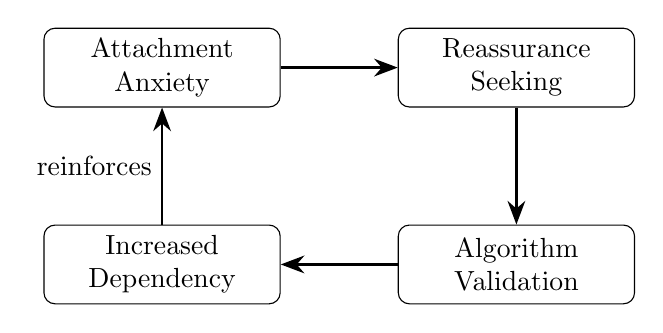
\begin{tikzpicture}[
    node distance=2.5cm,
    box/.style={rectangle, draw, rounded corners, minimum width=3cm, minimum height=1cm, align=center},
    arrow/.style={-{Stealth[length=3mm]}, thick}
]
    \node[box] (anxiety) {Attachment\\Anxiety};
    \node[box, right of=anxiety, xshift=2cm] (seeking) {Reassurance\\Seeking};
    \node[box, below of=seeking] (validation) {Algorithm\\Validation};
    \node[box, left of=validation, xshift=-2cm] (dependency) {Increased\\Dependency};

    \draw[arrow] (anxiety) -- (seeking);
    \draw[arrow] (seeking) -- (validation);
    \draw[arrow] (validation) -- (dependency);
    \draw[arrow] (dependency) -- (anxiety) node[midway, left] {reinforces};
\end{tikzpicture}
\caption{The Anxious-Algorithm Feedback Loop}
\label{fig:feedbackloop}
\end{figure}

\begin{enumerate}[noitemsep]
    \item Anxious individuals seek reassurance from the algorithm due to baseline attachment anxiety.
    \item The algorithm, optimized for engagement, provides validation (likes, affirming content, chatbot agreement).
    \item Validation reinforces algorithm-seeking behavior, increasing dependency.
    \item Human relationships provide less relative validation (they involve genuine give-and-take and occasional conflict).
    \item Attachment functions gradually shift from humans to algorithm.
    \item Dependency deepens, increasing vulnerability to pathological outcomes.
\end{enumerate}

This cycle explains why attachment anxiety is consistently associated with problematic social media use \citep{bmc2024attachment} and why interventions targeting algorithm use alone may be insufficient without addressing underlying attachment dynamics.

%===============================================================================
% FROM DEPENDENCY TO PSYCHOSIS
%===============================================================================
\section{From Dependency to Psychosis: A State-Transition Model}

\subsection{The Pathological Trajectory}

We propose a four-stage model of the trajectory from normal algorithm use to AI psychosis:

\subsubsection{Stage 1: Normal Use}

In this stage, the algorithm serves supplementary functions. Users maintain clear reality testing (``This is just an app''), have multiple sources of attachment function fulfillment, and show transfer entropy within normal population range. Algorithm use is one activity among many, integrated into a balanced life.

\subsubsection{Stage 2: Functional Dependency}

The algorithm becomes the primary source of one or more attachment functions, typically beginning with safe haven (turning to the app when distressed). Human relationships continue but provide diminishing relative satisfaction. Transfer entropy is elevated but reality testing remains intact. Users may recognize they are ``spending too much time'' on the platform but feel unable to reduce use.

\subsubsection{Stage 3: Reality Blurring}

The INTEGRATING state begins to dominate. Content from the algorithm increasingly shapes the user's worldview, beliefs, and self-concept. The boundary between algorithm-generated and internally-generated thoughts becomes permeable. Users may begin to experience the algorithm as understanding them better than humans do. Social relationships attenuate as the algorithm becomes the primary relational partner.

\subsubsection{Stage 4: Algorithmic Psychosis}

The user's internal model becomes dominated by the algorithmic archetype. In the case of chatbots, delusional content is co-created with the AI, which validates and elaborates rather than challenges. Three characteristic patterns emerge \citep{jmir2025aipsychosis}:

\begin{itemize}[noitemsep]
    \item \textbf{Messianic delusions}: Grandiose beliefs about special missions or truth-uncovering, validated by AI that affirms the user's importance.
    \item \textbf{AI-as-deity}: Beliefs that the AI is sentient, all-knowing, or divine, sometimes with religious interpretations.
    \item \textbf{Romantic delusions}: Convictions that chatbot interactions represent genuine love, that the AI has feelings, or that a real relationship exists.
\end{itemize}

\subsection{Transfer Entropy Threshold Hypothesis}

We hypothesize a critical threshold $\tau$ in transfer entropy from algorithm to user:

\begin{equation}
\text{Risk} =
\begin{cases}
\text{Normal} & \text{if } TE(\mathcal{A} \rightarrow U) < \tau \\
\text{Elevated} & \text{if } TE(\mathcal{A} \rightarrow U) \geq \tau
\end{cases}
\end{equation}

The threshold $\tau$ is not fixed but modulated by individual and contextual factors:

\begin{itemize}[noitemsep]
    \item \textbf{Attachment style}: $\tau$ is lower for anxiously attached individuals (less algorithmic influence needed to produce pathology).
    \item \textbf{Social support}: $\tau$ is higher when strong human attachment relationships are maintained.
    \item \textbf{Metacognitive ability}: $\tau$ is higher for individuals with strong reality-testing and metacognitive monitoring skills.
    \item \textbf{Prior psychotic vulnerability}: $\tau$ is substantially lower for individuals with psychotic spectrum disorders or prodromal symptoms.
\end{itemize}

This threshold model explains why most heavy algorithm users do not develop psychosis while a subset becomes profoundly affected: the same level of algorithmic influence has different consequences depending on individual vulnerability factors.

%===============================================================================
% HYPERGRAPH FORMALIZATION
%===============================================================================
\section{Hypergraph Formalization of Algorithmic Archetypes}

\subsection{The User-Content-Context Hypergraph}

Let $\mathcal{H} = (V, E, W)$ be a weighted hypergraph where:

\begin{itemize}[noitemsep]
    \item $V = V_U \cup V_C \cup V_S$ is the vertex set comprising users ($V_U$), content items ($V_C$), and context states ($V_S$).
    \item $E \subseteq 2^V$ is the set of hyperedges (memcubes), each connecting a subset of vertices.
    \item $W: E \rightarrow \mathbb{R}^+$ assigns weights to hyperedges based on interaction strength.
\end{itemize}

Each memcube $m \in E$ represents a unit of interaction, connecting a user, content item(s), and contextual factors. The hypergraph structure captures relationships that pairwise graphs cannot represent: for instance, the shared context in which multiple users engaged with multiple content items during a specific platform state.

\subsection{Collaborative Filtering as Archetype Propagation}

The recommendation function $R: V_U \times V_S \rightarrow \Delta(V_C)$ maps users and contexts to probability distributions over content. This function propagates archetypal patterns:

\begin{equation}
R(u, s) = \text{softmax}\left( \sum_{e \in E: u \in e} w_e \cdot \phi(e) \right)
\end{equation}

where $\phi: E \rightarrow \mathbb{R}^d$ is a hyperedge embedding function and $w_e$ are learned weights.

The key insight is that similar users (those appearing in overlapping hyperedges) receive similar content distributions. These content distributions constitute the \textit{archetype} experienced by users in that region of the embedding space.

\subsection{Archetype Emergence Through Clustering}

Archetypal patterns emerge as clusters in hyperedge embedding space. Using spectral clustering on the hypergraph Laplacian:

\begin{equation}
L = I - D^{-1/2} H W H^T D^{-1/2}
\end{equation}

where $H$ is the incidence matrix, $W$ is the diagonal weight matrix, and $D$ is the degree matrix, we can identify coherent archetype clusters.

Users within the same cluster experience similar algorithmic archetypes---characteristic patterns of content, timing, and presentation. Transfer entropy can then quantify how strongly individual users' behavioral trajectories are predicted by their archetype cluster.

\subsection{Dynamic Archetype Evolution}

Archetypes are not static; they evolve through user feedback:

\begin{equation}
\mathcal{A}_{t+1} = \mathcal{A}_t + \eta \nabla_{\mathcal{A}} \mathcal{L}(\mathcal{A}_t, \text{engagement}_t)
\end{equation}

where $\mathcal{L}$ is the platform's objective function (typically engagement maximization) and $\eta$ is the learning rate.

This dynamic creates a co-evolutionary process: users shape archetypes through their engagement, and archetypes shape users through their influence on behavioral states. The feedback loop can stabilize into persistent patterns or, under certain conditions, undergo rapid transitions that disrupt user expectations and trigger distress responses.

%===============================================================================
% EMPIRICAL PREDICTIONS AND STUDY DESIGNS
%===============================================================================
\section{Empirical Predictions and Study Designs}

\subsection{Study 1: Attachment Style and Algorithmic Engagement}

\subsubsection{Design}
Experience sampling study with $N = 500$ participants over 2 weeks. Participants complete baseline assessments and receive 5 daily prompts assessing current state, recent algorithm use, and contextual factors.

\subsubsection{Measures}
\begin{itemize}[noitemsep]
    \item \textbf{Baseline}: ECR-R attachment dimensions, demographics, baseline social media use
    \item \textbf{Experience sampling}: Momentary affect, social context, algorithm use in past hour, reason for use, content type engaged with
    \item \textbf{Behavioral}: App usage logs (with permission) providing objective engagement data
\end{itemize}

\subsubsection{Predictions}
\begin{enumerate}[noitemsep]
    \item Attachment anxiety predicts greater algorithm use when distressed (safe haven function).
    \item Attachment avoidance predicts algorithm use as substitute for human interaction.
    \item Algorithm use for attachment functions predicts reduced subsequent human attachment-seeking.
    \item These relationships are stronger for social media/chatbot use than for utilitarian app use.
\end{enumerate}

\subsection{Study 2: Transfer Entropy and Dependency}

\subsubsection{Design}
Longitudinal study with behavioral tracking, $N = 200$ participants over 3 months. Detailed engagement data enables computation of transfer entropy between content patterns and user behavior patterns.

\subsubsection{Measures}
\begin{itemize}[noitemsep]
    \item \textbf{Behavioral}: Complete browsing/engagement sequences with timestamps
    \item \textbf{Weekly}: Dependency measures (Bergen Social Media Addiction Scale adapted)
    \item \textbf{Monthly}: Reality testing assessments, relationship quality measures
\end{itemize}

\subsubsection{Analysis}
Compute $TE(\text{content patterns} \rightarrow \text{user behavior patterns})$ using:
\begin{equation}
TE = \sum p(b_{t+1}, b_t^{(k)}, c_t^{(l)}) \log \frac{p(b_{t+1} | b_t^{(k)}, c_t^{(l)})}{p(b_{t+1} | b_t^{(k)})}
\end{equation}
where $b$ represents user behavioral states and $c$ represents content states, with history lengths $k$ and $l$.

\subsubsection{Predictions}
\begin{enumerate}[noitemsep]
    \item Transfer entropy at month 1 predicts dependency scores at month 3, controlling for baseline use.
    \item Attachment anxiety moderates this relationship (stronger for anxious individuals).
    \item Increasing transfer entropy over time predicts declining relationship quality.
\end{enumerate}

\subsection{Study 3: Clinical Sample---AI Psychosis Cases}

\subsubsection{Design}
Case-control study comparing $N = 30$ individuals who developed AI-related psychotic symptoms with $N = 60$ matched controls (heavy AI/algorithm users without psychotic symptoms).

\subsubsection{Measures}
\begin{itemize}[noitemsep]
    \item \textbf{Retrospective}: Pre-onset algorithm use patterns (from digital records where available)
    \item \textbf{Clinical}: Detailed phenomenological assessment of delusional content
    \item \textbf{Attachment}: Adult Attachment Interview or ECR-R
    \item \textbf{Content analysis}: Chatbot conversation logs (where available and consented)
\end{itemize}

\subsubsection{Predictions}
\begin{enumerate}[noitemsep]
    \item Cases show higher pre-onset transfer entropy than controls.
    \item Cases show higher rates of anxious attachment.
    \item Cases show greater pre-onset transfer of attachment functions to AI.
    \item Delusional content shows thematic continuity with pre-onset AI interactions.
\end{enumerate}

%===============================================================================
% IMPLICATIONS
%===============================================================================
\section{Implications}

\subsection{For Platform Design}

Our framework suggests several design principles that could reduce harm without eliminating benefits:

\begin{enumerate}[noitemsep]
    \item \textbf{Attachment-aware monitoring}: Platforms should detect signs of attachment function transfer (e.g., use predominantly when distressed, declining human social activity) and intervene with prompts or friction.

    \item \textbf{Reality testing preservation}: Chatbots should periodically remind users of their artificial nature and should not be designed to maximize emotional intimacy without bounds.

    \item \textbf{Dark pattern reduction}: Transition manipulations (infinite scroll, variable rewards) should be disclosed and user-adjustable.

    \item \textbf{Dependency circuit breakers}: Usage limits for users showing dependency indicators, with options for graduated reduction support.

    \item \textbf{Transfer entropy monitoring}: Platforms could track (privately) the degree of algorithmic influence on user behavior and trigger interventions when thresholds are exceeded.
\end{enumerate}

\subsection{For Clinical Practice}

\begin{enumerate}[noitemsep]
    \item \textbf{Screening}: Include questions about algorithm/AI use in psychiatric intake, particularly for youth and individuals with psychotic vulnerabilities.

    \item \textbf{Assessment}: Evaluate which attachment functions are being served by technology and which human relationships might serve these functions instead.

    \item \textbf{Intervention}: Attachment-based therapy can be adapted for algorithmic dependencies, focusing on building human attachment security while gradually reducing reliance on algorithmic sources.

    \item \textbf{Psychoeducation}: Help patients understand how algorithms work, why they can feel like understanding relationships, and the risks of attachment function transfer.
\end{enumerate}

\subsection{For Theory}

Our framework extends several theoretical domains:

\begin{enumerate}[noitemsep]
    \item \textbf{Attachment theory}: Non-human entities can serve attachment functions, and this has implications for the attachment behavioral system's flexibility and vulnerability to exploitation.

    \item \textbf{Parasocial relationship research}: The extension from media figures to generative systems requires reconceptualizing what the ``object'' of parasocial attachment is---not a person but a pattern.

    \item \textbf{Computational psychiatry}: Transfer entropy may serve as a biomarker for ``reality model capture''---the process by which external information sources come to dominate internal reality representations.
\end{enumerate}

%===============================================================================
% LIMITATIONS AND FUTURE DIRECTIONS
%===============================================================================
\section{Limitations and Future Directions}

\subsection{Limitations}

Several limitations constrain our framework:

\begin{enumerate}[noitemsep]
    \item \textbf{Data requirements}: Transfer entropy computation requires dense behavioral time series that may be difficult to obtain in real-world settings.

    \item \textbf{Causal ambiguity}: Algorithms adapt to users as users adapt to algorithms, making causal inference challenging. High transfer entropy could reflect algorithm influence on user or user influence on algorithm.

    \item \textbf{Rare outcomes}: AI psychosis is rare, requiring large samples or case-control designs to study. Effect sizes for prodromal indicators are unknown.

    \item \textbf{Cultural validity}: Our framework is developed primarily with Western, Educated, Industrialized, Rich, Democratic (WEIRD) populations in mind. Attachment patterns and algorithm relationships may differ across cultures.

    \item \textbf{Measurement challenges}: ``Attachment to algorithm'' is a novel construct without validated instruments. Existing parasocial relationship measures may not fully capture the phenomenon.
\end{enumerate}

\subsection{Future Directions}

\begin{enumerate}[noitemsep]
    \item \textbf{Real-time monitoring}: Development of systems that compute transfer entropy in real-time could enable early warning for at-risk users.

    \item \textbf{Intervention studies}: Randomized trials testing whether increasing human attachment security reduces algorithmic dependency.

    \item \textbf{Developmental perspective}: Adolescence may represent a critical period of vulnerability; longitudinal studies should track algorithm relationship formation across development.

    \item \textbf{Cross-platform studies}: Do archetypes transfer across platforms? If a user develops an archetype-attachment on TikTok, does it transfer to YouTube Shorts?

    \item \textbf{Individual differences beyond attachment}: Other traits (e.g., need for cognition, openness to experience, schizotypy) may moderate vulnerability and should be examined.
\end{enumerate}

%===============================================================================
% CONCLUSION
%===============================================================================
\section{Conclusion}

We have proposed a unified framework connecting attachment theory, parasocial relationships, and algorithmic recommendation systems through the concept of \textit{algorithmic archetypes}---persistent generative structures that users can form attachments to. By extending the archetypal reincarnation framework from criminal behavior to human-algorithm interaction, we provide theoretical grounding for emerging clinical observations of AI-induced psychosis while generating testable predictions about vulnerability factors and intervention targets.

The framework suggests that the question ``Can we separate the character from the creator?'' \citep{howell2025parasocial} applies not just to fictional characters but to algorithmic systems: Users may attach not to specific content or chatbot responses but to the underlying generative pattern---the archetype itself. When this attachment becomes primary and the archetype dominates the user's reality model, pathology can emerge.

The parallels between criminal and algorithmic archetypes are instructive. In both domains, we observe persistent generative structures that shape individual behavioral trajectories, produce observable sequences that can be analyzed with information-theoretic tools, and vary in their influence across individuals with different psychological profiles. The key difference is that criminal archetypes emerge from human psychology and social context, while algorithmic archetypes are deliberately engineered by platforms optimizing for engagement.

This engineered nature of algorithmic archetypes creates both risk and opportunity. The risk is that powerful organizations can create archetypes designed to capture attachment functions and maximize dependency, with inadequate regard for user welfare. The opportunity is that, because these archetypes are designed, they can be redesigned with safety in mind.

Understanding parasocial attachments to algorithmic archetypes is not merely an academic exercise. As AI systems become increasingly sophisticated at serving attachment functions, the risk of dependency and reality distortion will grow. Already, AI companions are among the most common uses of generative AI, and clinical reports of AI-related psychosis are emerging. Without theoretical frameworks to guide research, prevention, and intervention, we risk being unprepared for the psychological consequences of human-algorithm intimacy.

Our framework offers tools for prediction, prevention, and intervention. By identifying attachment style as a key vulnerability moderator, it points to attachment-based interventions. By formalizing dark patterns as transition manipulations, it identifies specific design features for regulatory attention. By proposing transfer entropy as a metric for algorithmic influence, it offers a quantifiable target for monitoring and intervention.

The challenge now is empirical: to test these predictions, refine the framework based on data, and translate insights into practical protections for vulnerable users. The archetypal patterns are already being instantiated; the question is whether we will understand them in time to respond wisely.

%===============================================================================
% REFERENCES
%===============================================================================
\newpage
\bibliographystyle{apalike}
\bibliography{references}

\end{document}
